%!TEX program = xelatex
\documentclass[12pt, compress]{beamer}
\usetheme{Szeged}
\usecolortheme{beaver}

\usepackage{booktabs}
\usepackage[scale=2]{ccicons}
\usepackage[utf8]{inputenc}

%Font1:
%\usepackage{sansmathfonts}
%\usepackage[T1]{fontenc}
%\renewcommand*\familydefault{\sfdefault}
%Font2:
\usepackage[light,condensed,math]{kurier}
\usepackage[T1]{fontenc}

\usepackage{graphicx}

\newcommand{\titleA}{Introduction to Our Data Set}
\newcommand{\titleB}{Our Approach}
\newcommand{\titleC}{Sequential Minimal Optimization (SMO)}
\newcommand{\titleD}{Multi-Class Classification}
\newcommand{\titleE}{Results \& Conclusions}

\newtheorem{algorithm}{Algorithm}
\DeclareMathOperator{\argmax}{argmax}
\DeclareMathOperator{\argmin}{argmin}    

\title{Digit Recognition}
\subtitle{with Support Vector Machines}
\date{\today}
\author{Lisa \textsc{Gaedke-Merzh{\"a}user} \\% Your name
			Paul \textsc{Korsmeier}\\
			Lisa \textsc{Mattrisch}\\
			Vanessa \textsc{Schreck}\\}
\institute{Freie Universit{\"a}t Berlin, Mathematical Aspects of Machine Learning}


\begin{document}
\maketitle

\begin{frame}
  \frametitle{Outline} 
  \begin{enumerate}
	  \item \titleA
	  \item \titleB
	  \item \titleC
	  \item \titleD
	  \item \titleE
  \end{enumerate}
\end{frame}


\begin{frame}
  \frametitle{\titleA}
	\textbf{\alert{Main Goal:}} train algorithm to recognize handwritten digits
	\begin{figure}[h]
		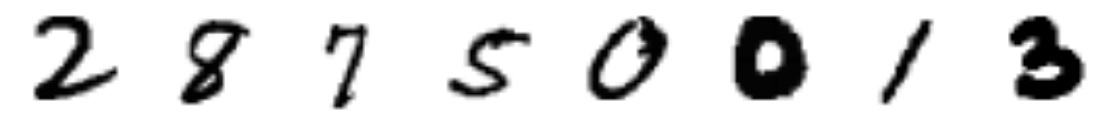
\includegraphics[width=1\textwidth]{Digits2}
		%\caption{Visualization of eight of the data points}
	\end{figure}
	\textbf{\alert{Data:}}
	\begin{itemize}
		\item 42,000 greyscale images
		\item 28 by 28 pixels each
		\item partitioned into ten classes
	\end{itemize}
\end{frame}


\begin{frame}
	\frametitle{\titleB}
	We want to use the concept of SVMs.
	
	\begin{figure}[h]
		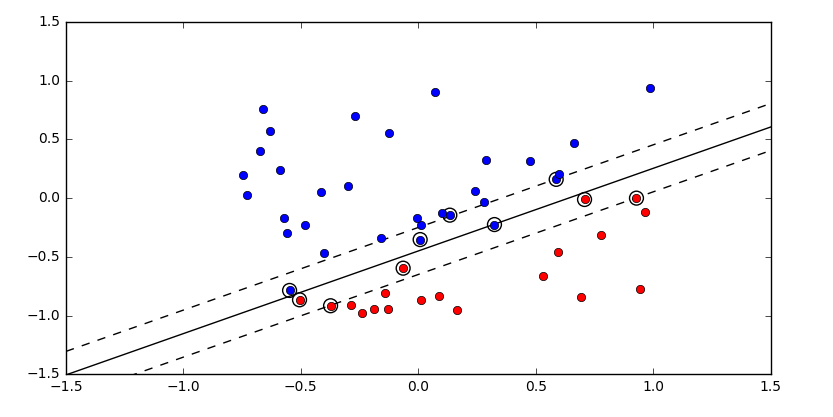
\includegraphics[width=0.7\textwidth]{svm_examplegraphic}
	\end{figure}
	
	
	\begin{itemize}
		\item \textbf{Problem I:} SVMs are binary classifiers 
		%\item We focus on two different approaches: 
		%\begin{enumerate}
		%	\item One-vs-All 
		%	\item Error-Correcting Output Codes
		%\end{enumerate}
		\item \textbf{Problem II:} Need to solve optimization problem
	\end{itemize}

\end{frame}


\begin{frame}
	\frametitle{\titleB}
	\begin{enumerate}
		\item Implement solver for our QP
		\begin{itemize}
			\item 3 versions
		\end{itemize}
		\item Implement basic SVM algorithm
		\begin{itemize}
			\item linear kernel / Gaussian kernel
			\item Parameter optimization
		\end{itemize}
		\item Combine individual SVMs in different ways
		\begin{itemize}
			\item 3 versions
		\end{itemize}
		\item Validate and compare results 
		\
	\end{enumerate}
\end{frame}

\begin{frame}
  \frametitle{\titleC}
  \begin{itemize}
  	\item The primal Soft Margin SVM QP is equivalent to solving the \textbf{\alert{dual problem:}}
  	\begin{eqnarray*}\label{eq:dual_problem}
  	\text{minimize} & d(\alpha) := \frac{1}{2} \alpha^T Q \alpha - 1^T \alpha  \\ 
  	\nonumber
  	\text{s.t.} &  0 \leq \alpha \leq C  \quad \text{and} \quad 	y^T \alpha = 0,
  	\end{eqnarray*}
  	where $q_{ij} = y_i y_j k(x_i,x_j)$, $x_i$ the data, $y_i$ the labels, $k$ the kernel function and $C$ the penalty term
  	\item Since Q is spsd, satisfying the KKT conditions guarantees a solution to (\ref{eq:dual_problem}).
  \end{itemize}
\end{frame}

\begin{frame}
\frametitle{\titleC}
\begin{itemize}
	
	\item Lagrangian of dual objective $d$: $\mathcal{L}(\alpha,\delta,\mu,\beta) = d(\alpha) - \delta^T\alpha + \mu^T(\alpha - C) - \beta \alpha^T y$
	\item \textbf{\alert{KKT conditions}} for dual Lagrangian:
	\begin{equation*}
	\left.
	\begin{aligned}
	\nabla_{\alpha} \mathcal{L}(\alpha^*,\delta^*,\mu^*,\beta^*) &= 0\\
	\delta_i^* &\geq 0\\
	\delta_i^* \alpha_i^* &= 0\\
	\mu_i^* &\geq 0\\
	\mu_i^* (\alpha_i^*-C) &= 0\\
	\alpha_i^* &\text{ feasible}
	\end{aligned}
	\right\} \text{for all } i \in \{1,\ldots,l\}
	\end{equation*}
	\item Define $F_i(\alpha) := y_i (\partial_i d)(\alpha) = \sum_{i = 1}^l \alpha_j y_j k(x_i,x_j) - y_i$.
\end{itemize}
\end{frame}

\begin{frame}
\frametitle{\titleC}
\begin{itemize}
	
	\item The KKT conditions are equivalent to:
	\begin{equation*}\label{equiv_KKT}
	b_{up}(\alpha) := \min_{i \in I_{up}(\alpha)} F_i(\alpha) \geq \max_{j \in I_{low}(\alpha)} F_j(\alpha) =: b_{low}(\alpha),
	\end{equation*}
	where $I_{up}(\alpha), I_{low}(\alpha) \subset \{1,\ldots,l\}$: \begin{itemize}
		\item $I_{up}(\alpha) := \{ i \mid  \alpha_i < C, y_i = 1 \text{ or } \alpha_i > 0, y_i = -1 \}$
		\item $I_{low}(\alpha) := \{ j \mid \alpha_j < C, y_j = -1 \text{ or } \alpha_j > 0, y_j = 1 \}$.
	
	\end{itemize}
	\item Relax to $b_{up}(\alpha) \geq b_{low}(\alpha) - \tau$ for some tolerance $\tau > 0$.
	\item A pair $(i,j) \in I_{up}(\alpha) \times I_{low}(\alpha)$ with $F_i(\alpha) < F_j(\alpha) - \tau$ is called \textbf{\alert{$\tau$-violating. }}
\end{itemize}
\end{frame}


\begin{frame}
\frametitle{\titleC}
	\begin{itemize}
		\item Any algorithm of the following form converges after finitely many steps:
	\end{itemize}
	\begin{algorithm}[General SMO type algorithm]\label{GSMO} Let $\tau > 0$. Initialize $k = 0 $ and $\alpha^0 = 0$ and generate iterates $\alpha^k$, $k \in \mathbb{N},$ as follows: 
		\begin{enumerate}
			\item If $\alpha^k$ satisfies $b_{up}(\alpha^k) \geq b_{low}(\alpha^k) - \tau$, stop. Else \textbf{\alert{pick}} a $\tau$-violating pair $(i,j) \in I_{up}(\alpha^k) \times I_{low}(\alpha^k)$.
			\item \textbf{\alert{Minimize}} $d$ only in $\alpha^k_i$ and $\alpha^k_j$, leaving $\alpha^k_n$ fixed for $n \notin \{i,j\}$ and respecting constraints. $\rightarrow$ Obtain \textbf{\alert{$\alpha^{\text{new}}$}}.
			\item Set $k := k+1$, $\alpha^k := \alpha^{\text{new}}$ and go to Step 1.
		\end{enumerate}
	\end{algorithm}
\end{frame}

\begin{frame}
\frametitle{\titleC}
\begin{itemize}
	\item Each step of GSMO is only a (clipped) \textbf{\alert{one-dimensional QP}} $\rightarrow$ analytic solution known $\rightarrow$ \textbf{\alert{cheap}}.
	\item Two heuristics for choosing violating pair: \\
	\begin{itemize}
		\item WSS1: steepest possible \textbf{\alert{gradient}}
		\[
		(i_{up},j_{low}) \in \argmin_{i \in I_{up}(\alpha)}F_i(\alpha) \times \argmax_{j \in I_{low}(\alpha)}F_j(\alpha)
		\]
		\item WSS2: maximal possible \textbf{\alert{decrease}} in $d$
		\[
		(i,j) \in \argmin_{i \in I_{up}(\alpha)}F_i(\alpha) \times I_{low}(\alpha): d(\alpha^{new}) - d(\alpha) \rightarrow \min
		\]
		
	\end{itemize}
	\item WSS2 seems promising, but is too expensive.
\end{itemize}
\end{frame}

\begin{frame}
	\frametitle{\titleC}
	
		\begin{itemize}
		\item \textbf{\alert{Run time comparison}} of algorithms with Gaussian kernel and labels by first ECOC classifier on our digits:
		\end{itemize}

	\begin{figure}[h]
	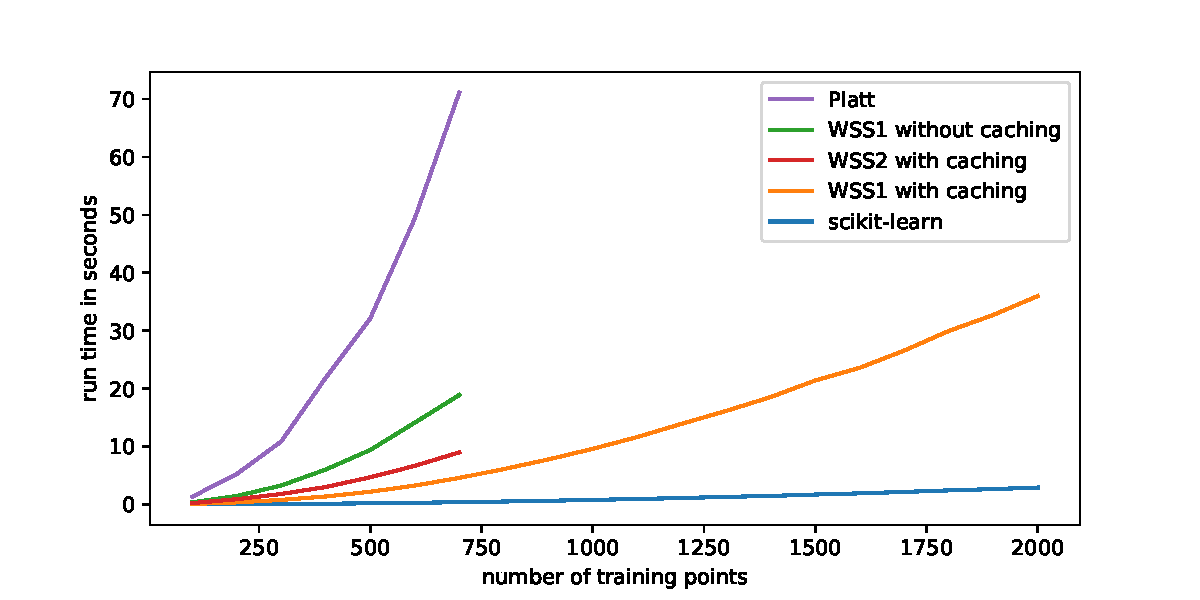
\includegraphics[width=1\textwidth]{images_for_presentation/benchplot_gauss.pdf}
	\end{figure}

\end{frame}

\begin{frame}
\frametitle{\titleC}
\begin{itemize}
	\item All algorithms seem to have \textbf{\alert{polynomial order 2.}}
	\item Our WSS1 with caching runs about 5.8 times as long as scikit-learn SVC.
\end{itemize}
\begin{figure}[h]
	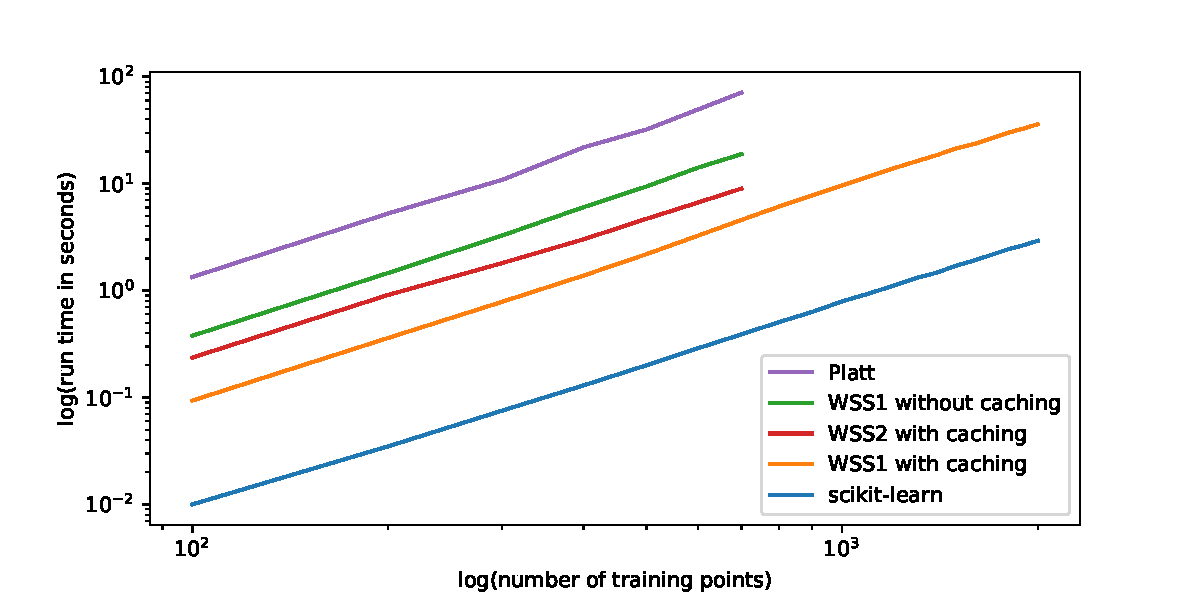
\includegraphics[width=1\textwidth]{images_for_presentation/benchplot_gauss_loglog.pdf}
\end{figure}
\end{frame}
          

\begin{frame}
  \frametitle{\titleD}
	\begin{itemize}
		\item Choose $k$ groups of the classes
		\item Train $k$ SVMs that separate each group from the rest
		\item Compare outcome to what would arise for each digit.
		\item \textbf{\alert{Problem:}} Points may not be classified uniquely.
		\item Handle overlappings by minimizing distance to barycenters
	\end{itemize}

	\begin{figure}[h]
		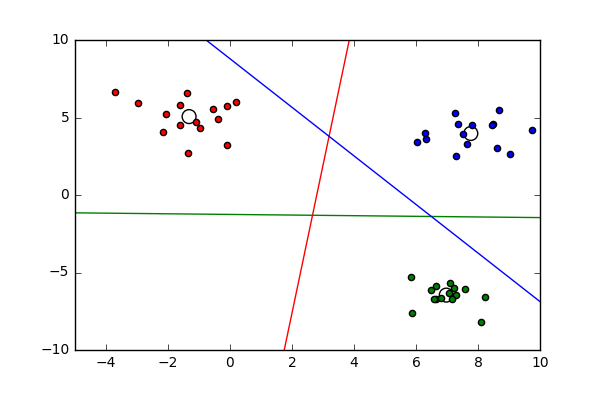
\includegraphics[width=.6\textwidth]{onevsall_examplegraphic}
		%\caption{Visualization of the One-vs-All approach}
	\end{figure}
\end{frame}

\begin{frame}
  \frametitle{\titleD}
	\textbf{\alert{1. One-vs-All}}\\
	\textbf{Idea:} For each $i \in \{0,1,\ldots,9\}$, train an SVM that separates class $i$ from the rest
  	\begin{table}[ht!]
		\centering
		\scalebox{0.8}{\begin{tabular}{|c|r|r|r|r|r|r|r|r|r|r|}
	\hline
	Class	& $f_0$ & $f_1$ & $f_2$ & $f_3$ & $f_4$ & $f_5$ & $f_6$ & $f_7$ & $f_8$ & $f_9$ \\ \hline \hline
	0	& -1 &  1 &  1 &  1 &  1 &  1 &  1 &  1 &  1 &  1 \\ \hline
	1	&  1 & -1 &  1 &  1 &  1 &  1 &  1 &  1 &  1 &  1 \\ \hline
	2	&  1 &  1 & -1 &  1 &  1 &  1 &  1 &  1 &  1 &  1 \\ \hline
	3	&  1 &  1 &  1 & -1 &  1 &  1 &  1 &  1 &  1 &  1 \\ \hline
	4	&  1 &  1 &  1 &  1 & -1 &  1 &  1 &  1 &  1 &  1 \\ \hline
	5	&  1 &  1 &  1 &  1 &  1 & -1 &  1 &  1 &  1 &  1 \\ \hline
	6	&  1 &  1 &  1 &  1 &  1 &  1 & -1 &  1 &  1 &  1 \\ \hline
	7	&  1 &  1 &  1 &  1 &  1 &  1 &  1 & -1 &  1 &  1 \\ \hline
	8	&  1 &  1 &  1 &  1 &  1 &  1 &  1 &  1 & -1 &  1 \\ \hline
	9	&  1 &  1 &  1 &  1 &  1 &  1 &  1 &  1 &  1 & -1 \\ \hline
\end{tabular}}
	\end{table} 
\end{frame}



\begin{frame}
  \frametitle{\titleD}
	\textbf{\alert{2. Error Correcting Output Codes}}\\
	\textbf{Idea:} Relabeling with large Hamming distance according to:
	\begin{table}[ht!]
		\centering
		\scalebox{0.8}{\begin{tabular}{|c|l|l|l|l|l|l|l|l|l|l|l|l|l|l|l|}
	\hline
	Class	& $f_0$ & $f_1$ & $f_2$ & $f_3$ & $f_4$ & $f_5$ & $f_6$ & $f_7$ & $f_8$ & $f_9$ & $f_{10}$ & $f_{11}$ & $f_{12}$ & $f_{13}$ & $f_{14}$ \\ \hline \hline
	0	& 1 & 1 & -1 & -1 & -1 & -1 & 1 & -1 & 1 & -1 & -1 & 1 & 1 & -1 & 1 \\ \hline
	1	& -1 & -1 & 1 & 1 & 1 & 1 & -1 & 1 & -1 & 1 & 1 & -1 & -1 & 1 & -1 \\ \hline
	2	& 1 & -1 & -1 & 1 & -1 & -1 & -1 & 1 & 1 & 1 & 1 & -1 & 1 & -1 & 1 \\ \hline
	3	& -1 & -1 & 1 & 1 & -1 & 1 & 1 & 1 & -1 & -1 & -1 & -1 & 1 & -1 & 1 \\ \hline
	4	& 1 & 1 & 1 & -1 & 1 & -1 & 1 & 1 & -1 & -1 & 1 & 1 & -1 & -1 & 1 \\ \hline
	5	& -1 & 1 & -1 & -1 & 1 & 1 & -1 & -1 & 1 & 1 & -1 & -1 & -1 & -1 & 1 \\ \hline
	6	& 1 & -1 & 1 & 1 & 1 & -1 & -1 & -1 & -1 & 1 & -1 & 1 & -1 & -1 & 1 \\ \hline
	7	& -1 & -1 & -1 & 1 & 1 & 1 & 1 & -1 & 1 & -1 & 1 & 1 & -1 & -1 & 1 \\ \hline
	8	& 1 & 1 & -1 & 1 & -1 & 1 & 1 & -1 & -1 & 1 & -1 & -1 & -1 & 1 & 1 \\ \hline
	9	& -1 & 1 & 1 & 1 & -1 & -1 & -1 & -1 & 1 & -1 & 1 & -1 & -1 & 1 & 1 \\ \hline
\end{tabular}}
	\end{table}  
\end{frame}



\begin{frame}
  \frametitle{\titleE}
	\begin{table}[ht!]
		\centering
		\scalebox{0.7}{
		\begin{tabular}{|l|l|l|l|l|l|l|l|l|l|l|l|} \hline
			\multicolumn{1}{|p{1.8cm}|}{\vspace*{.7 cm}\# training points} &
			\multicolumn{1}{p{1.8cm}|}{\vspace*{0 cm}\hbox{One-vs-All} uniquely classfied, linear} &
			\multicolumn{1}{p{1.8cm}|}{\vspace*{0 cm}\hbox{One-vs-All} with bary- centers, linear} &
			\multicolumn{1}{p{1.8cm}|}{\vspace*{0 cm}\hbox{One-vs-All} uniquely classfied, Gaussian} &
			\multicolumn{1}{p{1.8cm}|}{\vspace*{0 cm}\hbox{One-vs-All} with bary-centers, Gaussian} &
			\multicolumn{1}{p{1.8cm}|}{\vspace*{.7 cm}ECOC, \hbox{linear}} &
			\multicolumn{1}{p{1.8cm}|}{\vspace*{.7 cm}ECOC, Gaussian} \\ \hline \hline
			500	& \visible<2->{65.9\%} & \visible<2->{74.1\%} & \visible<2->{75.4\%} & \visible<2->{83.3\%} & \visible<2->{74.2\%} & \visible<2->{87.4\%} \\ \hline
1000	& \visible<2->{68.2\%} & \visible<2->{75.0\%} & \visible<2->{84.3\%} & \visible<2->{89.0\%} & \visible<2->{78.0\%} & \visible<2->{92.7\%} \\ \hline
2000	& \visible<2->{70.2\%} & \visible<2->{76.4\%} & \visible<2->{89.8\%} & \visible<2->{91.9\%} & \visible<2->{77.8\%} & \visible<2->{94.3\%} \\ \hline
5000	& \visible<2->{70.0\%} & \visible<2->{73.8\%} & \visible<2->{88.9\%} & \visible<2->{91.6\%} & \visible<2->{82.0\%} & \visible<2->{95.2\%} \\ \hline
10000	& \visible<2->{64.6\%} & \visible<2->{67.5\%} & \visible<2->{88.0\%} & \visible<2->{90.6\%} & \visible<2->{82.5\%} & \visible<2->{95.4\%} \\ \hline
		\end{tabular}
		}
		\caption{Correctly Classified Digits}
	\end{table}
\end{frame}

\begin{frame}
  \frametitle{\titleE}
	\begin{figure}[h]
		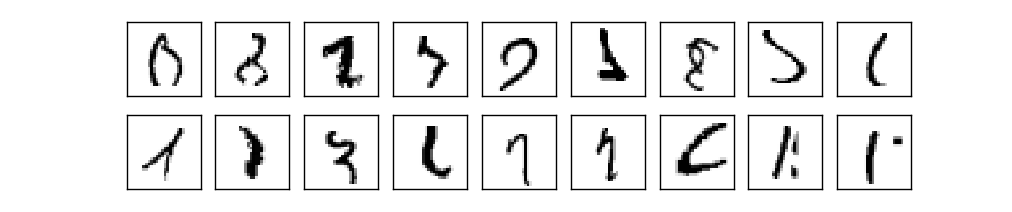
\includegraphics[width=1\textwidth]{mnist_really_bad_images}
		\caption{Visualizing very illegible digits}
	\end{figure}
\end{frame}

\end{document}

